\section{Minimizing Robust Loss Using an ERM Oracle \label{erm}}
\label{sec:non-realizable-oracle}

First, we show an example where the approach of \citet{xiang2022patchcleanser} of calling $\ERM_\calH$ on the inflated dataset, i.e., original training points plus all possible perturbations resulting from the allowed masking operations, fails by obtaining %
a multiplicative gap of $k-1$ %
in the robust loss between the optimal robust classifier and the classifer returned by $\ERM_\calH$, where $k$ is the size of the perturbation sets. This gap exists since $\ERM$ can exhibit a solution that incorrectly classifies at least one perturbation per natural example, while there is a robust classifier that concentrates error on one natural example, thus getting low robust loss.

\begin{exmpl}
\label{exmpl:ERM-failure}
Consider the following example in $\mathcal{R}$. There is a training set $\{z_1,\cdots,z_{2n}\}$ of original examples, where examples $\{z_1,\cdots,z_n\}$ are positively labeled and are located at $x=1$. $\{z_{n+1},\cdots,z_{2n}\}$ are negatively labeled and are at $x=-1$. Each example $z_i$ has $k=n$ perturbations denoted by $\{z_{i,1},\cdots,z_{i,k}\}$. 

For each of the negative examples $\{z_{n+1},\cdots,z_{2n-1}\}$, all their perturbations are at $x=-0.75$. For the negative example $z_{2n}$, all its perturbations, i.e. $\{z_{2n,1},\cdots,z_{2n,k}\}$, are at $x=0$. For each positive example $z_i$ where $i\in\{1,\cdots,n-1\}$, one of their perturbations $z_{i,1}$ is at $x=0$ and the rest, i.e. $\{z_{i,2},\cdots,z_{i,k}\}$, are at $x=0.75$. For the positive example $z_n$, all its perturbations $z_{n,1},\cdots,z_{n,k}$ are at $x=0.75$.

 The adversarial training procedure considered in the paper by~\citet{xiang2022patchcleanser} runs ERM on the augmented dataset (original examples and all their perturbations) to minimize the 0/1 loss. ERM finds a threshold classifier $h_{ERM}$ with threshold $\tau=\eps_1$ for any $0<\eps_1<0.75$ that classifies any points with $x<\tau$ as negative and points with $x\geq \tau$ as positive. As a result, for each positive example $z_i$ for $i\in\{1,\cdots,n-1\}$, the perturbation $z_{i,1}$ is getting classified mistakenly which causes a robust loss on $z_i$. Therefore, $h_{ERM}$ has a robust loss of $(n-1)/2n$  since $n-1$ of the positive examples are not robustly classified. 
However, there exists a threshold classifier $h^*$ with threshold $\tau=\eps_2$ for any $-0.75<\eps_2<0$ that only makes mistakes on perturbations of $z_{2n}$ and thus has a robust loss of $1/2n$. However, its 0/1 loss is higher than $h_{ERM}$ and therefore ERM does not pick it.
Therefore, ERM can be suboptimal up to a multiplicative factor of $n-1$ for any arbitrary value of $n$. An illustration is given in~\prettyref{fig:example}.


\begin{figure}[ht]
\label{fig:example}
\centering
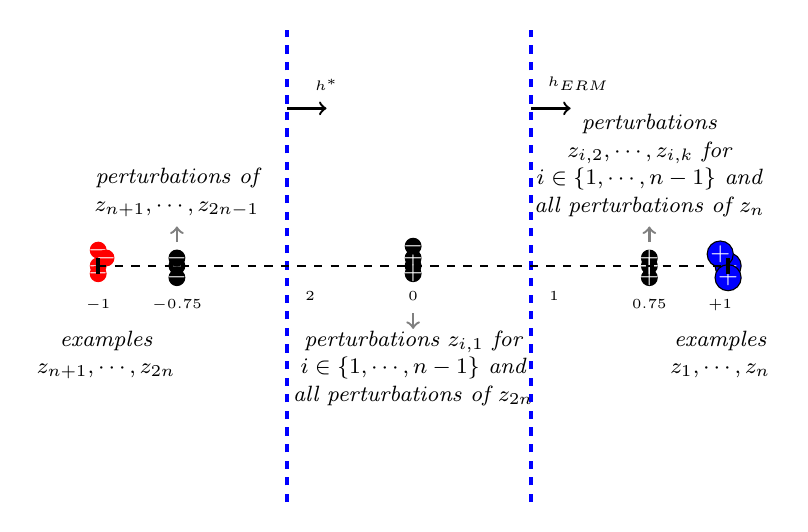
\begin{tikzpicture}%


 \draw[red, fill=red,text=white] (-4,0) circle (0.1cm);
 \node[white] at (-4,0) {\small{$-$}};

 \draw[red, fill=red,text=white] (-4,0.2) circle (0.1cm);
 \node[white] at (-4,0.2) {\small{$-$}};

 \draw[red, fill=red,text=white] (-3.9,0.1) circle (0.1cm);
 \node[white] at (-3.9,0.1) {\small{$-$}};

 \draw[red, fill=red,text=white] (-4,-0.1) circle (0.1cm);
 \node[white] at (-4,-0.1) {\small{$-$}};
 
 \draw[line width=0.5mm] (-4,-0.1) -- (-4,0.1);
 \node[below] at (-4,-0.3) {\tiny{$-1$}};
 \node[below,align=center,font=\fontsize{8}{10}\itshape\selectfont] at (-3.9,-0.7) {examples\\ $z_{n+1},\cdots,z_{2n}$};
 
\draw[black, fill=black,text=white] (-3,0) circle (0.1cm);
\node[white] at (-3,0) {\small{$-$}};

 \draw[black, fill=black,text=white] (-3,0.1) circle (0.1cm);
\node[white] at (-3,0.1) {\small{$-$}};

 \draw[black, fill=black,text=white] (-3,-0.15) circle (0.1cm);
\node[white] at (-3,-0.15) {\small{$-$}};
\node[below] at (-3,-0.3) {\tiny{$-0.75$}};
\node[above,align=center,font=\fontsize{8}{10}\itshape\selectfont] at (-3,0.5) {perturbations of\\ $z_{n+1},\cdots,z_{2n-1}$};
\draw[->,line width=0.3mm,gray] (-3,0.3)--(-3,0.5);
\draw[black, fill=black,text=white] (+3,0) circle (0.1cm);
\node[white] at (+3,0) {\small{$+$}};

 \draw[black, fill=black,text=white] (+3,0.1) circle (0.1cm);
\node[white] at (+3,0.1) {\small{$+$}};

 \draw[black, fill=black,text=white] (+3,-0.15) circle (0.1cm);
\node[white] at (+3,-0.15) {\small{$+$}};
\node[below] at (+3,-0.3) {\tiny{$0.75$}};
\node[above,align=center,font=\fontsize{8}{10}\itshape\selectfont] at (+3,0.5) {perturbations \\ $z_{i,2},\cdots,z_{i,k}$ for\\ $i\in\{1,\cdots,n-1\}$ and\\ all perturbations of $z_n$};
\draw[->,line width=0.3mm,gray] (3,0.3)--(3,0.5);

\draw[black, fill=black,text=white] (0,0) circle (0.1cm);
\node[white] at (+3,0) {\small{$+$}};

 \draw[black, fill=black,text=white] (0,0.1) circle (0.1cm);
\node[white] at (0,0.1) {\small{$+$}};

 \draw[black, fill=black,text=white] (0,-0.1) circle (0.1cm);
\node[white] at (0,-0.1) {\small{$+$}};

 \draw[black, fill=black,text=white] (0,0.25) circle (0.1cm);
\node[white] at (0,0.25) {\small{$-$}};



\node[below] at (0,-0.2) {\tiny{$0$}};
\node[above,align=center,font=\fontsize{8}{10}\itshape\selectfont] at (0,-1.9) {perturbations $z_{i,1}$ for\\ $i\in\{1,\cdots,n-1\}$ and\\ all perturbations of $z_{2n}$};

\draw[->,line width=0.3mm,gray] (0,-0.6)--(0,-0.8);
\node[circle,draw, minimum size = 0.1cm, inner sep=0pt,fill=blue] (C) at  (+4,0) [text=white] {\small{+}};

\node[circle,draw, minimum size = 0.1cm, inner sep=0pt,fill=blue] (C) at  (+3.9,0.15) [text=white] {\small{+}};

\node[circle,draw, minimum size = 0.1cm, inner sep=0pt,fill=blue] (C) at  (+4,-0.15) [text=white] {\small{+}};
\node[below] at (3.9,-0.3) {\tiny{$+1$}};
\node[below,align=center,font=\fontsize{8}{10}\itshape\selectfont] at (3.9,-0.7) {examples\\ $z_{1},\cdots,z_{n}$};

\draw[line width=0.5mm] (4,-0.1) -- (4,0.1);

\draw[line width=0.5mm,blue,dashed] (1.5,-3) -- (1.5,3);
\node[below] at (1.8,-0.2) {\tiny{$\eps_1$}};

\draw[->,line width=0.3mm] (1.5,2) -- (2,2);
\node[above] at (2.1,2.1) {\tiny{$h_{\text{ERM}}$}};

\draw[line width=0.5mm,blue,dashed] (-1.6,-3) -- (-1.6,3);
\node[below] at (-1.3,-0.2) {\tiny{$\eps_2$}};

\draw[->,line width=0.3mm] (-1.6,2) -- (-1.1,2);
\node[above] at (-1.1,2.1) {\tiny{$h^*$}};

\draw[dashed, line width=0.2mm] (-4,0) -- (4,0);

\end{tikzpicture}
\caption{
$\ERM$ failure mode in the robustly un-realizable case. Blue, red, and black points show respectively original examples with a positive label, original examples with a negative label, and perturbations of original examples.
}
\end{figure}
\end{exmpl}

Next, we present our first contribution: %
we show in~\prettyref{thm:generalization-FMS} that~\prettyref{alg:FMS} proposed by 
~\citet{DBLP:conf/colt/FeigeMS15} learns a predictor that is simultaneously robust to a set of (polynomially many) masking operations, using an $\ERM_\calH$ oracle. The algorithm is based on prior work%
, but the analysis and application are novel in this work. A detailed comparison with~\citet{DBLP:conf/colt/FeigeMS15} is given in~\prettyref{sec:feigecomparison}. The main interesting feature of this algorithm is that it achieves stronger robustness guarantees in the non-realizable regime when $\OPT_\calH \gg 0$, where the approach of \citet{xiang2022patchcleanser} can fail as mentioned in~\prettyref{exmpl:ERM-failure}. 

\begin{algorithm}%
\begin{algorithmic}[1]
\caption{\citet*{DBLP:conf/colt/FeigeMS15}}
\label{alg:FMS}
  \INPUT weight update parameter $\eta>0$, number of rounds $T$, and training dataset $S=\{(x_1,y_1),\dots, (x_m,y_m)\}$ and corresponding weights $p_1,\cdots,p_m$\;
  
  \STATE 
  Set $w_1(z, (x,y)) = 1$, for each $(x,y)\in S, z\in \calU(x)$.\;
  
  \STATE 
  Set $P^1(z,(x,y)) = \frac{w_1(z,(x,y))}{\sum_{z'\in\calU(x)} w_1(z',(x,y))}$, for each $(x,y)\in S, z\in \calU(x)$.\;
  
\FOR{each $t\in \{1,\cdots T\}$}%
\STATE 
Call $\ERM$ on the empirical weighted distribution:\;
\STATE 
{\small\[h_t = \argmin_{h\in\mathcal{H}} \sum_{(x,y)\in S} \sum_{z\in \calU(x)} {p_{(x,y)} }P^t(z,(x,y)) \ind\insquare{h_{t}(z)\neq y}\]}\;
\FOR{each $(x,y)\in S$ and $z\in\calU(x)$}%
\STATE {\small $w_{t+1}(z,(x,y)) = (1+\eta \ind\insquare{h_{t}(z)\neq y}) \cdot w_{t}(z, (x,y))$}\;

\STATE 
$P^{t+1}(z,(x,y))=\frac{w_t(z,(x,y))}{\sum_{z'\in\calU(x)} w_t(z',(x,y))}$\;
\ENDFOR
\ENDFOR
\OUTPUT The majority-vote predictor $\MAJ(h_1,\dots, h_T)$. \\
\end{algorithmic}
\end{algorithm}





\begin{thm}
\label{thm:generalization-FMS}
Set $T(\eps) = \frac{32 \ln k}{\eps^2}$ and $m(\eps, \delta) = O\inparen{\frac{\vc(\calH)(\ln k)^2}{\eps^4}\ln \inparen{\frac{\ln k}{\eps^2}}+\frac{\ln(1/\delta)}{\eps^2}}$. Then, for any distribution $\calD$ over $\calX\times \calY$, with probability at least $1-\delta$ over $S\sim \calD^{m(\eps,\delta)}$, running \prettyref{alg:FMS} {where $p_{(x,y)}=1/m$ for all $(x,y)\in S$ }for $T(\eps)$ rounds produces $h_1,\dots,h_{T(\eps)}$ satisfying:

\small\[\Ex_{(x,y)\sim \calD} \insquare{ \max_{z\in \calU(x)} \ind\insquare{\MAJ(h_1,\dots, h_{T(\eps)})(z)\neq y} } 
\leq 2\OPT_{\calH} + \eps\]
where $\MAJ(h_1,\dots, h_{T(\eps)})$ shows the majority-vote of predictors $h_1,\dots, h_{T(\eps)}$.
\end{thm}

\begin{rem}
In the approach proposed by~\citet{xiang2022patchcleanser}, the robust loss with respect to the (exponentially many) patches is upper bounded by the robust loss with respect to the (polynomially many) masking operations. Therefore,~\prettyref{thm:generalization-FMS} implies that the robust loss against patches is at most $2\OPT_{\calH} + \eps$.
\end{rem}

\subsection{Comparison with prior related work} 
\label{sec:feigecomparison}
As presented, \cite{DBLP:conf/colt/FeigeMS15} only considered \emph{finite} hypothesis classes $\calH$ and provided generalization guarantees depending on $\log\abs{\calH}$. On the other hand, we consider here infinite classes $\calH$ with bounded VC dimension and provide tighter robust generalization bounds (see \prettyref{thm:generalization-FMS}). We would also like to highlight another difference. Given an output of $h_1,\dots,h_T$ from \prettyref{alg:FMS}, the guarantee provided by \cite{DBLP:conf/colt/FeigeMS15} is on average and does not exactly capture the notion of robust loss %
i.e. the loss on input $x$ is $\sup_{z\in\calU(x)} \frac{1}{T}\sum_{t=1}^{T} \ind[h_t(z)\neq y]$ (\prettyref{lem:FMS} states their result). We emphasize that this is different from the \emph{robust loss} guarantee that we obtain in~\prettyref{thm:generalization-FMS} for a %
single classifier, i.e. the loss on input 
$x$ is captured as $\sup_{z\in\calU(x)} \ind[\MAJ(h_1,\dots,h_T)(z)\neq y]$. %
In particular, unlike the %
guarantee provided by \cite{DBLP:conf/colt/FeigeMS15} in which the adversary chooses $z\in\calU(x)$ and then we can probabilistically choose a classifier to classify it, to implement the Patch-Cleanser reduction we need a single classifier that is \emph{simultaneously} correct on \emph{all} 
$z\in\calU(x)$. Because of the difference in guarantees derived, we incur a multiplicative factor of 2 compared with their bound. 

The robust learning guarantee \citep[][Theorem 2]{attias2022improved} assumes access to a \emph{robust} $\ERM$ oracle, which minimizes the robust loss on the training dataset. On the other hand, at the expense of higher sample complexity, we provide a robust learning guarantee using only an $\ERM$ oracle which is a more common and simpler assumption in the challenging \emph{non-realizable} setting. Prior work due to \citet{DBLP:conf/nips/MontasserHS20} considered using an $\ERM$ oracle for robust learning but only in the simpler realizable setting (when $\OPT_\calH=0$).


\subsection{Proof of \prettyref{thm:generalization-FMS}}
We exhibit a sketch for the proof of~\prettyref{thm:generalization-FMS} and defer the details to the Appendix. The main insight is to solve a finite zero-sum game. In particular, our goal is to find a mixed-strategy over the hypothesis class that is approximately close to the value of the game:
\[\OPT_{S,\calH} \triangleq \min_{h\in \calH} \frac{1}{m}\sum_{i=1}^{m} \max_{z_i\in \calU(x_i)} \ind\insquare{h(z_i)\neq y_i}.\]
 

We observe that \prettyref{alg:FMS} due to \citep{DBLP:conf/colt/FeigeMS15} solves a similar finite zero-sum game (see \prettyref{lem:FMS}), and then we relate it to the value of the game we are interested in (see \prettyref{lem:opt}). Combined together, this only establishes that we can minimize the robust loss on the empirical dataset using an $\ERM$ oracle. We then appeal to uniform convergence guarantees for the robust loss in \prettyref{lem:unif-robloss} to show that, with a large enough training data, our output predictor achieves robust risk that is close to the value of the game. 

\begin{lem}
\label{lem:opt}
For any dataset $S %
=\{(x_1,y_1),\dots,(x_m,y_m)\}\in (\calX\times\calY)^m$ {with corresponding weights $p_1,\cdots,p_m=1/m$},
\begin{align*}
    &\OPT_{S,\calH} = \min_{h\in \calH} \frac{1}{m}\sum_{i=1}^{m} \max_{z_i\in \calU(x_i)} \ind\insquare{h(z_i)\neq y_i} \\
    &\geq
    \min_{Q\in \Delta(\calH)} \max_{\substack{P_{1}\in \Delta(\calU(x_1)),\\ \dots\\ P_{m} \in \Delta(\calU(x_m))}} \frac{1}{m} \sum_{i=1}^{m} \Ex_{z_i\sim P_i } \Ex_{h\sim Q} \ind\insquare{h(z_i)\neq y_i}
\end{align*}
\end{lem}




\begin{lem} [\citet*{DBLP:conf/colt/FeigeMS15}]
\label{lem:FMS}
For any data set $S %
=\{(x_1,y_1),\dots,(x_m,y_m)\}\in (\calX\times\calY)^m$ {with corresponding weights $p_1,\cdots,p_m=1/m$}, running \prettyref{alg:FMS} for $T$ rounds produces a mixed-strategy $\hat{Q} = \frac{1}{T} \sum_{t=1}^{T} h_t \in \Delta(\calH)$ satisfying:
{\small
\begin{align*}
    &\max_{\substack{P_1\in \Delta(\calU(x_1)),\\ \dots,\\ P_m\in \Delta(\calU(x_m))}} \frac{1}{m}\sum_{i=1}^{m} \Ex_{z_i\sim P_i} \frac{1}{T} \sum_{t=1}^{T} \ind\insquare{h_t(z_i)\neq y_i} \\
    &\leq
    \min_{Q\in \Delta(\calH)} \max_{\substack{P_{1}\in \Delta(\calU(x_1)),\\ \dots,\\ P_{m} \in \Delta(\calU(x_m))}} \frac{1}{m} \sum_{i=1}^{m} \Ex_{z_i\sim P_i } \Ex_{h\sim Q} \ind\insquare{h(z_i)\neq y_i} + 
    2\sqrt{\frac{\ln k}{T}}
\end{align*}
}%
\end{lem}


\removed{
\begin{lem} [Extension to weighted samples]
For any data set $S %
=\{(x_1,y_1),\dots,(x_m,y_m)\}\in (\calX\times\calY)^m$ and any corresponding weights $p_1,\dots, p_m > 0$ such that $\sum_{i=1}^{m} p_i = 1$, running \prettyref{alg:FMS} for $T$ rounds produces a mixed-strategy $\hat{Q} = \frac{1}{T} \sum_{t=1}^{T} h_t \in \Delta(\calH)$ satisfying:
\begin{align*}
    \max_{P_1\in \Delta(\calU(x_1)),\dots,P_m\in \Delta(\calU(x_m))} &\sum_{i=1}^{m} p_i\cdot \Ex_{z_i\sim P_i} \frac{1}{T} \sum_{t=1}^{T} \ind\insquare{h_t(z_i)\neq y_i} \leq\\
    &\min_{Q\in \Delta(\calH)} \max_{P_{1}\in \Delta(\calU(x_1)),\dots, P_{m} \in \Delta(\calU(x_m))} \sum_{i=1}^{m} p_i\cdot \Ex_{z_i\sim P_i } \Ex_{h\sim Q} \ind\insquare{h(z_i)\neq y_i} + 2\sqrt{\frac{\ln k}{T}}.
\end{align*}
\label{lem:extension-FMS-weights}
\end{lem}
}


\begin{lem} [VC Dimension for the Robust Loss \citep{attias2022improved}]
\label{lem:unif-robloss}
For any class $\calH$ and any $\calU$ such that $\sup_{x\in\calX}\abs{\calU(x)}\leq k$, denote the robust loss class of $\calH$ with respect to $\calU$ by
\[\calL^{\calU}_{\calH} = \{(x,y)\mapsto \max_{z\in\calU(x)} \ind\insquare{h(z)\neq y}: h\in\calH\}.\]
Then, it holds that $\vc(\calL^{\calU}_{\calH})\leq O(\vc(\calH) \log(k))$. 
\end{lem}


